\chapter{Aufbau der Fallstudie}
\label{sec:fallstudie}

Im Rahmen dieser Masterarbeit soll nun mithilfe von Hadoop und der Selfbalancing"=Komponente eine Fallstudie durchgeführt werden, durch die ermittelt wird, unter welchen Umständen eine Testautoamtisierung möglich ist.
Dazu werden zunächst Anforderungen an das Hadoop"=System selbst gestellt, die es im Rahmen dieser Tests erfüllen soll.
Neben diesen funktionalen Anforderungen werden aber auch Anforderungen an das Testsystem selbst gestellt, die durch die Tests selbst erfüllt sein sollen.
Zur Realisierung dieser Tests wird für das reale Cluster die von \citeauthor{zhang2016} entwickelte Plattform Hadoop"=Benchmark genutzt.

\section{Anforderungen an das Cluster und Testsystem}
\label{sec:requirements}

Zur Überprüfung des Clusters und des Testssystems selbst werden hierfür jeweils mehrere Anforderungen gestellt.
Unterschieden wird hierbei zwischen funktionalen Anforderungen an das \gls{SuT} und Anforderungen an das Testsystem.
Während die funktionalen Anforderungen ausschließlich vom Hadoop"=Cluster als \gls{SuT} erfüllt werden müssen, müssen die Test"=Anforderungen vom gesamten Testsystem erfüllt werden.

Mithilfe der im Folgenden definierten Anforderungen soll bereits automatisiert geprüft werden, inwieweit eine Testautomatisierung möglich ist.
Hierfür werden die Anforderungen, sofern möglich, in Form von Constraints ebenfalls im Modell implementiert und während der Ausführung durch das Oracle validiert.

\subsection{Funktionale Anforderungen an das Cluster}
\label{subsec:functionalRequirements}

Obwohl in dieser Masterarbeit der Fokus auf Testautomatisierung und Validieren eines Testsystems liegt, müssen auch die funktionalen Anforderungen an das \gls{SuT}, also das Hadoop"=Cluster selbst, berücksichtigt werden.
Da im Rahmen der Publikation \cite{Eberhardinger2018} ebenfalls der in \cref{sec:clusterSetup} beschriebene und in dieser Fallstudie genutzte Versuchsaufbau genutzt wurde, wurden im Rahmen dieser Fallstudie auch funktionale Anforderungen an das Cluster selbst durch das Oracle geprüft.
Dies betrifft konkret folgende Anforderungen an das \gls{SuT} \cite{Eberhardinger2018}:

\begin{enumerate}
    \item Ein Task wird vollständig ausgeführt, sofern er nicht abgebrochen wird
    \item Kein Task oder \gls{Anwendung} wird an inaktive, defekte oder nicht verbundene Nodes gesendet
    \item Die Konfiguration wird aktualisiert, sobald eine entsprechende Regel erfüllt ist
    \item Defekte oder Verbindungsabbrüche werden erkannt
\end{enumerate}

\subsection{Anforderungen an das Testsystem}
\label{subsec:testRequirements}

Neben den funktionalen Anforderungen, gibt es weitere Anforderungen an das gesamte Testsystem.
Diese Anforderungen betreffen das Hadoop"=Cluster, die Selfbalancing"=Komponente, das entwickelte \gls{ss}"=Modell sowie der Treiber zur Kommunikation zwischen Modell und Cluster.
Konkret sind dies folgende Anforderungen an das Testsystem:

\begin{enumerate}
    \item Der \gls{MARP}"=Wert ändert sich basierend auf den derzeit ausgeführten Anwendungen
    \item Der jeweils aktuelle Status des Clusters wird erkannt und im Modell gespeichert
    \item Defekte Nodes und Verbindungsabbrüche werden erkannt
    \item Im Modell implementierte Komponentenfehler werden im realen Cluster injiziert und repariert
    \item Wenn alle Nodes defekt sind, wird erkannt, dass sich das Cluster nicht mehr rekonfigurieren kann
    \item Ein \gls{Test} kann vollautomatisch ausgeführt werden
    \item Das Cluster kann ohne Auswirkungen auf seine Funktionsweise auf einem oder mehreren Hosts ausgeführt werden
    \item Es können mehrere Benchmark\gls{Anwendung}en gleichzeitig gestartet und ausgeführt werden
    \item \glspl{Test} und \glspl{Testfall} können zeitlich unabhängig und mehrmals ausgeführt werden
\end{enumerate}

Die funktionalen Anforderungen dienen zudem ebenfalls als Anforderungen an das Testsystem und erweitern somit die hier genannten Anforderungen.

Eine Besonderheit bildet die fünfte Anforderung, wonach erkannt werden muss, dass im Cluster keine weitere Rekonfiguration möglich ist.
Wird diese Anforderung verletzt soll der ausgeführte \gls{Test} abgebrochen werden, während bei den anderen, auch den funktionalen, Anforderungen dies nur durch das Oracle vermerkt werden soll, die Ausführung aber nicht weiter beeinträchtigt werden soll.


\section{Anforderungen an das Testsystem}
\label{sec:evaluationPlan}

Um das Testsystem zu validieren, wurde zunächst ein Evaluationsplan aufgestellt.
In diesem ist festgehalten, was getestet wird, wie die Testfälle aussehen und wie die bei der Ausführung gewonnen Daten organisiert werden.

\subsection{Behauptungen und Variablen}
\label{sec:predictions}

% Was für Behauptungen wurden aufgestellt
\begin{enumerate}
    \setcounter{enumi}{4}
    \item Der jeweils aktuelle Status des Clusters wird erkannt und im Modell gespeichert
    \item Defekte Nodes und Verbindungsabbrüche werden erkannt
    \item Im Modell implementierte Komponentenfehler werden im realen Cluster injiziert und repariert
    \item Wenn alle Nodes defekt sind, wird erkannt, dass sich das Cluster nicht mehr rekonfigurieren kann
    \item Ein Test kann vollautomatisch ausgeführt werden
    \item Das Cluster kann ohne Auswirkungen auf die Funktionsweise auf einem oder beiden Hosts ausgeführt werden
    \item Es können mehrere Benchmark"=Anwendungen gleichzeitig gestartet und ausgeführt werden
    \item Ein Testfall kann zeitlich unabhängig und mehrmals ausgeführt werden
\end{enumerate}

% Was für Variablen wurden dadurch ermittelt

\subsection{Generierung der Testfälle}
\label{sec:testcaseGeneration}

Die Generierung der Testfälle hängt von mehreren Faktoren ab.
Zum einen ist ein Testfall abhängig von der Größe des Clusters, also ob das Cluster auf einem oder beiden Hosts ausgeführt wird und aus wie vielen Nodes das Cluster besteht.
Relevant zur Unterscheidung von Testfällen sind aber auch die ausgeführten Anwendungen.
Da die Auswahl der ausgeführten Anwendungen nicht manuell bestimmt werden soll, wird hierfür ein Transitionssystem verwendet.
Mithilfe dieses Transitionssystems, in dem die Wahrscheinlichkeiten von Wechsel zwischen zwei Anwendungen definiert sind, soll während der Ausführung eines Testfalls zufällig eine nachfolgende Anwendung ausgewählt werden.
Da zum Testen des Clusters der \ac{ss}"=Simulator eingesetzt wird, hängt die Anzahl der Anwendungen primär von der Anzahl der ausgeführten Simulations"=Schritte ab.
Ein weiterer Faktor zur Anzahl der Anwendungen ist die Anzahl an simulierten Clients, da auch getestet werden soll, wie sich das Cluster bei der Ausführung von mehreren parallel gestarteten Anwendungen verhält.
Die zu injizierenden Komponentenfehler, mit denen defekte Nodes und Verbindungsausfälle simuliert werden, werden ebenfalls zufallsbasiert ausgewählt.
Dies gilt auch für das Deaktivieren der Komponentenfehlern.

Die Auswahl der nachfolgenden Anwendungen und die Entscheidung über die Aktivierung und Deaktivierung der Komponentenfehlern wird daher mithilfe eines Zufallsgenerators realisiert.
Hierbei soll jedoch kein echter Zufallsgenerator zum Einsatz kommen, sondern ein Pseudo"=Zufallsgenerator.
Da ein Pseudo"=Zufallsgenerator seine Werte mithilfe eines Start"=\emph{Seeds} auswählt, besteht somit die Möglichkeit durch die Verwendung eines bestimmten Seeds, einen Testfall jederzeit wiederholen zu können.
Zur Auswahl der ersten Testfälle werden daher zeitbasierte Seeds verwendet.
Diese Seeds werden bei der Ausführung notiert und für andere Testfälle verwendet, bei denen andere Punkte der Konfiguration wie \zB die Größe des Clusters, abgeändert werden.
Dadurch ist es möglich, die Auswirkungen einzelner Parameter zu testen und zu evaluieren.
\todo{Wo wird Seed wie genutzt? am besten in implementierung davon!}

\subsection{Organisation und Ausgabe der Daten}
\label{sec:dataOrganisation}

Damit die bei der Ausführung gewonnenen Daten auch zur Evaluation genutzt werden können, wurde hierzu festgelegt, welche Daten während der Ausführung ausgegeben werden.
Alle relevante Daten werden hierzu während der Ausführung der Testfälle in einer Log"=Datei gespeichert.
Zur Unterscheidung von einzelnen Ausführungen werden die Daten klar strukturiert.
Neben den im folgenden beschriebenen Daten werden zudem alle Ein- und Ausgabedaten der SSH"=Verbindungen zwischen \ac{ss} und dem Cluster (vgl. \autoref{sec:aufbauCluster}) in einem eigenen Log gespeichert.

Beim Start der Simulation werden zunächst einige generelle Daten ausgegeben:

\begin{itemize}
    \item Basis"=Seed für die Zufallsgeneratoren
    \item Mindestdauer für einen Simulations"=Schritt
    \item Anzahl der ausgeführten Simulations"=Schritte
    \item Wahrscheinlichkeiten für Aktivierung und Deaktivierung der Komponentenfehler
    \item Angabe, ob vorab generierte Eingabedaten genutzt werden oder diese während der Ausführung eines Testfalls generiert werden
    \item Anzahl genutzter Hosts und Nodes
    \item Pfade verwendeter Scripte auf den Hosts (vgl. \autoref{sec:aufbauCluster})
    \item Bei der Nutzung der REST"=API verwendete URL des Controllers
    \item Auszuführende Benchmarks    
\end{itemize}

Die Ausgabe der Daten der YARN"=Komponenten wird bei jedem Simulations"=Schritt durchgeführt, damit das Verhalten des Clusters berücksichtigt werden kann.
Ausgegeben werde hierbei:

\begin{itemize}
    \item Für jeden Node:
    \begin{itemize}
        \item ID bzw. Name des Nodes
        \item Aktueller Status
        \item Informationen zur Fehleraktivierung
        \item Anzahl ausgeführter Container auf dem Node
        \item Angaben zur Speicherauslastung
        \item Angaben zur CPU"=Auslastung
    \end{itemize}
    
    \item Für jeden Client:
    \begin{itemize}
        \item ID bzw. Name des Clints
        \item Aktuell ausgeführter Benchmark
        \item ID der aktuell ausgeführten Anwendung auf dem Cluster
    \end{itemize}

    \item Für jede Anwendung:
    \begin{itemize}
        \item ID der Anwendung
        \item Bezeichnung der Anwendung
        \item Aktueller und finaler Status der Anwendung
        \item ID bzw. Name des Nodes, auf dem der \ac{AppMstr} ausgeführt wird
    \end{itemize}

    \item Für jeden Attempt:
    \begin{itemize}
        \item ID des Attempts
        \item Aktueller Status des Attempts
        \item ID des \ac{AppMstr}"=Containers
        \item ID bzw. Name des Nodes, auf dem der \ac{AppMstr} ausgeführt wird
    \end{itemize}

    \item Für jeden Container:
    \begin{itemize}
        \item ID des Containers
        \item ID bzw. Name des auszuführenden Nodes
        \item Aktueller Status des Containers
    \end{itemize}
\end{itemize}

Die Details zur Implementierung und dem Ausgabeformat sind in \autoref{sec:simulationStepOutput} erläutert.


\section{Umsetzung des realen Clusters}\label{sec:aufbauCluster}

\citeauthor{zhang2016} haben im Rahmen ihrer gesamten Forschungsarbeit die Open"=Source"=Plattform Hadoop"=Benchmark entwickelt und auf Github zur Verfügung gestellt.\footnote{\url{https://github.com/Spirals-Team/hadoop-benchmark}}
Sie wurde speziell zum Einsatz in der Forschung erstellt und kann jederzeit an die eigenen Bedürfnisse angepasst werden.
Auf Basis dieser Plattform und der enthaltenen Benchmarks wurde das reale Cluster für diese Masterarbeit aufgebaut.

\subsection{Plattform Hadoop"=Benchmark}\label{sec:hadoopBenchmark}

Die Plattform ist in mehrere Szenarien unterteilt, darunter ein Hadoop in der Version 2.7.1 ohne Änderungen und ein darauf basierendes Szenario mit der Selfbalancing"=Komponente.
Hadoop"=Benchmark basiert auf der Software \emph{Docker}\footnote{\url{https://www.docker.com/}} und dem dazugehörigen Tool \emph{Docker Machine}, um damit mit wenigen Befehlen ein Hadoop"=Cluster aufbauen zu können.
Mit \emph{Graphite}\footnote{\url{https://graphiteapp.org/}} ist zudem ein Monitoring"=Tool enthalten, mit dem die Systemwerte wie CPU- oder Speicher"=Auslastung des Clusters überwacht und analysiert werden kann.

\begin{figure}
    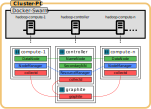
\includegraphics{./images/hadoopBenchmarkArch.png}
    \caption[High"=Level"=Architektur von Hadoop"=Benchmark]
    {High"=Level"=Architektur von Hadoop"=Benchmark.
        Entnommen aus \cite{abb:hadoopBenchmarkArch}.}
    \label{fig:hadoopBenchmarkArchitecture}
\end{figure}

\autoref{fig:hadoopBenchmarkArchitecture} zeigt die grundlegende Architektur der Plattform, die mithilfe eines Docker"=Swarms auf mehreren \emph{Docker Machines} ein Cluster erstellt, auf denen dann in den Docker"=Containern das eigentliche Hadoop"=Cluster ausgeführt wird.
In Hadoop"=Benchmark werden mithilfe von Docker"=Machine und VirtualBox\footnote{\url{https://www.virtualbox.org/}} virtuelle Maschinen erstellt, die mit dem  Betriebssystem \emph{Boot2Docker} ausgestattet sind.
Boot2Docker ist eine leichtgewichtige Linux"=Distribution, auf der Docker bereits vorinstalliert ist \cite{DockerMachineGettingStartedVm}.
Jeder Hadoop"=Container enthält zudem das Tool \emph{collectd}\footnote{\url{https://collectd.org/}}, was das Monitoring des Containers auf Systemebene übernimmt und die Daten an den Graphite"=Container übermittelt.
Dadurch wird es möglich, eine beliebige Anzahl an voneinander unabhängigen Nodes auf einem physischen Computer ausführen zu können.
Auch ist es möglich, den Docker"=Machines einen beliebig großen Arbeitsspeicher zur Verfügung zu stellen.

Die Plattform Hadoop"=Benchmark enthält zudem einige Benchmark"=Anwendungen:

\begin{itemize}
    \item Hadoop Mapreduce Examples
    \item Intel HiBench\footnote{\url{https://github.com/intel-hadoop/HiBench}}
    \item \ac{SWIM} \footnote{\url{https://github.com/SWIMProjectUCB/SWIM}}
\end{itemize}

Eine Besonderheit bildet der SWIM"=Benchmark, welcher sehr Ressourcenintensiv ist und daher auf einem \emph{Single Node Cluster}, also einem kompletten Hadoop"=Cluster auf nur einem Computer, sehr zeitintensiv sein kann.
Der Intel HiBench"=Benchmark besteht aus Kategorien wie \emph{Machine Learning} oder Graphen, welche wiederum aus einen oder mehreren \emph{Workloads} bestehen, welche entsprechende Anwendungen bzw. Algorithmen auf dem Hadoop"=Cluster ausführen.
Einige der Hibench"=Workloads basieren auf den Mapreduce Examples, welche wiederum voneinander unabhängige Beispielanwendungen für Hadoop darstellen.

\subsection{In dieser Fallstudie verwendetes Setup}\label{sec:clusterFallstudie}

Da die Plattform Hadoop"=Benchmark mithilfe von Docker auf einem physischen PC sehr einfach ein komplettes Hadoop"=Cluster ausführen kann, wurde die Plattform für diese Fallstudie als Basis genutzt.
Da Docker und Hadoop vor allem für den Einsatz in einer Linux"=Umgebung entwickelt wurden, werden für die Fallstudie zwei Computer genutzt, auf denen das Cluster wahlweise auf einem oder auf beiden Hosts ausgeführt werden kann.
Zudem wird auf einem Host eine VM mit Windows 10 ausgeführt, das zum Ausführen des .NET"=Frameworks bzw. \sS benötigt wird.
Beide zum Einsatz kommenden Hosts sind jeweils mit einem Intel Core i5"=4570 @ 3,2 GHz x 4, 16 GB Arbeitsspeicher sowie einer SSD ausgestattet, auf der Ubuntu 16.04 LTS installiert ist.
Die Verbindung von Windows zu Linux auf beiden Hosts wird mithilfe von SSH"=Verbindungen umgesetzt.

\begin{figure}
    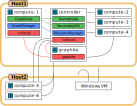
\includegraphics{./images/caseStudyHadoopSetup.pdf}
    \caption[In der Fallstudie verwendetes Cluster"=Setup]
    {In der Fallstudie verwendetes Cluster"=Setup.
        Grün: \ac{HDFS}, Blau: YARN, Rot: Graphite.}
    \label{fig:caseStudyHadoopSetup}
\end{figure}

\todo{Irgendwo erwähnen, wie Docker-Container aufeinander aufbauen}
Die beiden Abbildungen \autoref{fig:hadoopBenchmarkArchitecture} und \autoref{fig:caseStudyHadoopSetup} zeigen bereits den großen Hauptunterschied zwischen der Plattform und dem hier verwendeten Cluster"=Setup.
Da durch die Nutzung von virtuellen Maschinen ein zusätzlicher Ressourcenbedarf entsteht, wird im hier verwendeten Setup darauf verzichtet.
Durch die Ausführung der Docker"=Container des Hadoop"=Clusters direkt auf dem Host stehen dem Cluster mehr Ressourcen zur Verfügung.
Zudem wird es mithilfe von von \emph{Docker Swarm} so ermöglicht, das Hadoop"=Cluster auf beiden Hosts auszuführen.
Im konkreten Setup werden dabei Graphite, der Hadoop"=Controller sowie vier Hadoop"=Nodes auf dem Host1, sowie zwei weitere, optionale Nodes auf Host2 ausgeführt.
Weitere Anpassungen des verwendeten Setups bestehen \uA darin, dass der \ac{TLS} von Hadoop ebenfalls gestartet wird.
Zudem wurden einige Einstellungen von Hadoop so angepasst, dass defekte Nodes schneller erkannt werden.

Zum Ausführen der Windows"=VM auf Host2 wird VirtualBox 5.2 verwendet.
Zum Abrufen von Daten mithilfe der REST"=API von Hadoop über die SSH"=Verbindungen wird \emph{curl}\footnote{\url{https://curl.haxx.se/}} genutzt.
Zum Ausführen des Hadoop"=Clusters wird Docker in der Version 18.03 CE genutzt.

Um die in dieser Fallstudie benötigten Befehle einfach ausführen zu können, wurden zwei eigene Scripte erstellt, welche zum Teil auf den bestehenden Scripten der Plattform aufbauen.
Das Setup"=Script dient für folgende Zwecke:

\begin{itemize}
    \item Starten und Beenden des Clusters
    \item Starten und Beenden einzelner Hadoop"=Nodes
    \item Hinzufügen und Entfernen der Netzwerkverbindung des Docker"=Containers eines Hadoop"=Nodes
    \item Ausführen von eigenen Befehlen auf dem Docker"=Container des Hadoop"=Controllers
    \item Erstellen des Hadoop"=Docker"=Images
\end{itemize}

Das zweite erstellte Script dient ausschließlich zum Starten der Benchmarks.
Dazu werden die in der Plattform bereits enthaltenen Start"=Scripte aufgerufen, die für das konkrete Setup angepasst wurden.

